\documentclass[tikz,border=8pt]{standalone}
% Shared look for every TikZ diagram. Load with \input{../../tools/tikz-style.tex}
\usepackage[T1]{fontenc}
\usepackage{lmodern}
\renewcommand{\sfdefault}{lmr}  % diagrams use the same serif as the text
\usetikzlibrary{arrows.meta, positioning, shapes.geometric, calc, fit, backgrounds}
\definecolor{cblue}{HTML}{4C78A8}
\definecolor{corange}{HTML}{F58518}
\definecolor{cgreen}{HTML}{54A24B}
\definecolor{cred}{HTML}{E45756}
\definecolor{cpurple}{HTML}{B279A2}
\definecolor{cgrey}{HTML}{6B6B6B}
\tikzset{
  every picture/.style={font=\sffamily, line width=1.2pt},
  box/.style={draw=#1, fill=#1!12, rounded corners=4pt, align=center, inner sep=7pt, minimum height=1.1cm},
  box/.default=cgrey,
  arrow/.style={-{Stealth[length=3mm]}, draw=cgrey, line width=1.4pt},
  title/.style={font=\sffamily\bfseries\Large},
  note/.style={font=\sffamily\small, text=cgrey, align=center},
}
\AtBeginDocument{\hyphenpenalty=10000 \exhyphenpenalty=10000}

\begin{document}
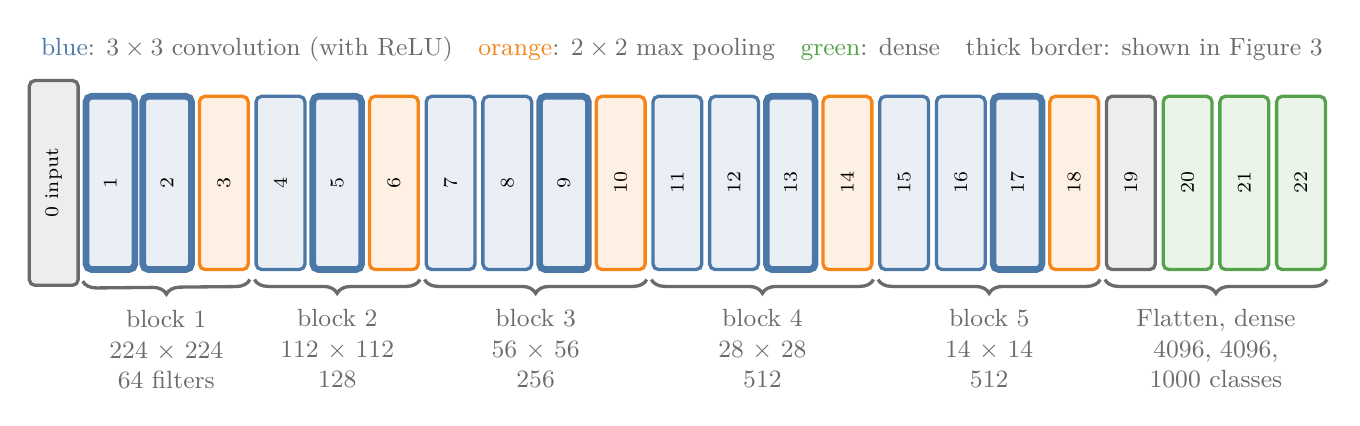
\begin{tikzpicture}[
    l/.style={draw=#1, fill=#1!12, rounded corners=2pt, minimum width=0.62cm, minimum height=2.2cm, inner sep=1pt,
              font=\sffamily\scriptsize},
    pick/.style={line width=2.4pt}]
  % position / colour / shown in the feature-map figure (1) or not (0)
  \foreach \i/\col/\s in {1/cblue/1, 2/cblue/1, 3/corange/0, 4/cblue/0, 5/cblue/1, 6/corange/0, 7/cblue/0, 8/cblue/0, 9/cblue/1, 10/corange/0, 11/cblue/0, 12/cblue/0, 13/cblue/1, 14/corange/0, 15/cblue/0, 16/cblue/0, 17/cblue/1, 18/corange/0, 19/cgrey/0, 20/cgreen/0, 21/cgreen/0, 22/cgreen/0} {
    \ifnum\s=1
      \node[l=\col, pick] (n\i) at (0.72*\i, 0) {\rotatebox{90}{\i}};
    \else
      \node[l=\col] (n\i) at (0.72*\i, 0) {\rotatebox{90}{\i}};
    \fi
  }
  \node[l=cgrey, minimum height=2.6cm] (in) at (0, 0) {\rotatebox{90}{0 input}};
  % block labels
  \foreach \a/\b/\t in {1/3/{block 1\\224 $\times$ 224\\64 filters}, 4/6/{block 2\\112 $\times$ 112\\128}, 7/10/{block 3\\56 $\times$ 56\\256},
                        11/14/{block 4\\28 $\times$ 28\\512}, 15/18/{block 5\\14 $\times$ 14\\512}} {
    \draw[decorate, decoration={brace, amplitude=5pt, mirror}, cgrey] ([yshift=-3pt]n\a.south west) -- ([yshift=-3pt]n\b.south east)
      node[midway, below=7pt, note, align=center] {\t};
  }
  \draw[decorate, decoration={brace, amplitude=5pt, mirror}, cgrey] ([yshift=-3pt]n19.south west) -- ([yshift=-3pt]n22.south east)
      node[midway, below=7pt, note, align=center] {Flatten, dense\\4096, 4096,\\1000 classes};
  \node[note, anchor=south west, align=left] at (-0.3, 1.4) {\textcolor{cblue}{blue}: $3 \times 3$ convolution (with ReLU)\quad
     \textcolor{corange}{orange}: $2 \times 2$ max pooling\quad \textcolor{cgreen}{green}: dense\quad thick border: shown in Figure 3};
\end{tikzpicture}
\end{document}
